
%(BEGIN_QUESTION)
% Copyright 2007, Tony R. Kuphaldt, released under the Creative Commons Attribution License (v 1.0)
% This means you may do almost anything with this work of mine, so long as you give me proper credit

The process trend shown below reveals a controller's response to the process variable signal and the setpoint.  Based on what you see in this trend, determine whether the controller is direct or reverse acting, and also whether it implements a P-only, I-only, or P+I control algorithm.

$$\includegraphics[width=15.5cm]{i01634x01.eps}$$

\vfil

\underbar{file i01634}
\eject
%(END_QUESTION)





%(BEGIN_ANSWER)

This is a graded question -- no answers or hints given!

%(END_ANSWER)





%(BEGIN_NOTES)

This is a {\bf reverse-acting, P+I} controller.  

\vskip 10pt

We can tell it exhibits ``P'' action because the output steps immediately as the SP steps.  We can also tell it exhibits ``I'' action because the output ramps as the error between PV and SP persists over time.  Its action is ``reverse'' because the direction of the output change is the same as the SP change (which implies it is opposite of the PV change, since the effects of PV and SP changes always oppose each other).

%INDEX% Control, proportional + integral: response of real controller to setpoint change

%(END_NOTES)


